\section{configobj::Template\-Interpolation Class Reference}
\label{classconfigobj_1_1TemplateInterpolation}\index{configobj::TemplateInterpolation@{configobj::TemplateInterpolation}}
Inheritance diagram for configobj::Template\-Interpolation::\begin{figure}[H]
\begin{center}
\leavevmode
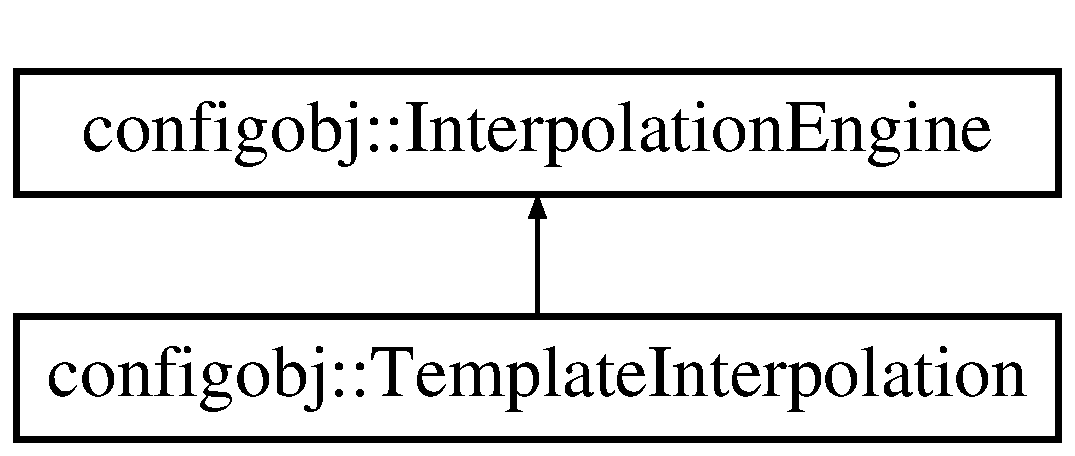
\includegraphics[height=2cm]{classconfigobj_1_1TemplateInterpolation}
\end{center}
\end{figure}


\subsection{Detailed Description}


\footnotesize\begin{verbatim}Behaves like string.Template.\end{verbatim}
\normalsize
 



The documentation for this class was generated from the following file:\begin{CompactItemize}
\item 
old/PANICtool-1.0/configobj.py\end{CompactItemize}
